%%%%%%%%%%%%%%%%%%%%%%%%%%%%%%%%%%%%%%%%%
% Classicthesis Typographic Thesis
% LaTeX Template
% Version 1.4 (1/1/16)
%
% This template has been downloaded from:
% http://www.LaTeXTemplates.com
%
% Original author:
% André Miede (http://www.miede.de) with commenting modifications by:
% Vel (vel@LaTeXTemplates.com)
%
% License:
% GNU General Public License (v2)
%
% General Tips:
% 1) Make sure to edit the classicthesis-config.file
% 2) New enumeration (A., B., C., etc in small caps): \begin{aenumerate} \end{aenumerate}
% 3) For margin notes: \marginpar or \graffito{}
% 4) Do not use bold fonts in this style, it is designed around them
% 5) Use tables as in the examples
% 6) See classicthesis-preamble.sty for useful commands
%
%%%%%%%%%%%%%%%%%%%%%%%%%%%%%%%%%%%%%%%%%

%----------------------------------------------------------------------------------------
%	PACKAGES AND OTHER DOCUMENT CONFIGURATIONS
%----------------------------------------------------------------------------------------

\documentclass[
		twoside,openright,titlepage,numbers=noenddot,headinclude,%1headlines,
	 	footinclude=true,cleardoublepage=empty,
		dottedtoc, % Make page numbers in the table of contents flushed right with dots leading to them
		BCOR=5mm,paper=a4,fontsize=11pt, % Binding correction, paper type and font size
		ngerman,american, % Languages, change this to your language(s)
		]{scrreprt} 
                
% Includes the file which contains all the document configurations and packages - make sure to edit this file
%%%%%%%%%%%%%%%%%%%%%%%%%%%%%%%%%%%%%%%%%
% Classicthesis Typographic Thesis
% Configuration File
%
% This file has been downloaded from:
% http://www.LaTeXTemplates.com
%
% Original author:
% André Miede (http://www.miede.de) with extensive commenting changes by:
% Vel (vel@LaTeXTemplates.com)
%
% License:
% GNU General Public License (v2)
%
% Important note:
% The main lines to change in this file are in the DOCUMENT VARIABLES
% section, the rest of the file is for advanced configuration.
%
%%%%%%%%%%%%%%%%%%%%%%%%%%%%%%%%%%%%%%%%%

%RSD: ADD PACKAGES AND DO YOUR OWN CONFIG TWEAKING HERE:
\usepackage{bm} % Might not be supported
\usepackage{amsmath}
\usepackage{ amssymb }

%%%%%%%%%%%%%%%%%%%%%%%%%%%%%%%%%%%%%%%%%%%%%%%%%%%%%%%%%


%\usepackage[euler-digits,euler-hat-accent]{eulervm}
\DeclareMathOperator{\argmax}{argmax}

%----------------------------------------------------------------------------------------
%	CHARACTER ENCODING
%----------------------------------------------------------------------------------------

\PassOptionsToPackage{utf8}{inputenc} % Set the encoding of your files. UTF-8 is the only sensible encoding nowadays. If you can't read äöüßáéçèê∂åëæƒÏ€ then change the encoding setting in your editor, not the line below. If your editor does not support utf8 use another editor!
\usepackage{inputenc}

%----------------------------------------------------------------------------------------
%	DOCUMENT VARIABLES
%	Fill in the lines below to enter your information into the thesis template
%	Each of the commands can be cited anywhere in the thesis
%----------------------------------------------------------------------------------------

% Remove drafting to get rid of the '[ Date - classicthesis version 4.0 ]' text at the bottom of every page
\PassOptionsToPackage{eulerchapternumbers,listings,drafting, pdfspacing, subfig,beramono,eulermath,parts}{classicthesis}
% Available options: drafting parts nochapters linedheaders eulerchapternumbers beramono eulermath pdfspacing minionprospacing tocaligned dottedtoc manychapters listings floatperchapter subfig

\newcommand{\myTitle}{Project Thesis in Nanotechnology at NTNU\xspace}
\newcommand{\mySubtitle}{Optimisation of Small Angle X-ray Scattering Tensor Tomography Gradient Descent Algorithm by Automatic Differentiation\xspace}
\newcommand{\myDegree}{Mr\xspace}
\newcommand{\myName}{Ruben Skjelstad Dragland\xspace}
\newcommand{\myProf}{Dag Werner Breiby\xspace}
\newcommand{\myOtherProf}{Basab Chattopadhyay\xspace}
\newcommand{\mySupervisor}{Dag Werner Breiby\xspace}
\newcommand{\myFaculty}{Faculty of Natural Sciences\xspace}
\newcommand{\myDepartment}{Department of Physics\xspace}
\newcommand{\myUni}{Norwegian University of Science and Technology\xspace}
\newcommand{\myLocation}{Trondheim\xspace}
\newcommand{\myTime}{December 2022\xspace}
\newcommand{\myVersion}{version 1.0\xspace}

%----------------------------------------------------------------------------------------
%	USEFUL COMMANDS
%----------------------------------------------------------------------------------------

\newcommand{\ie}{i.\,e.}
\newcommand{\Ie}{I.\,e.}
\newcommand{\eg}{e.\,g.}
\newcommand{\Eg}{E.\,g.}

\newcounter{dummy} % Necessary for correct hyperlinks (to index, bib, etc.)
\providecommand{\mLyX}{L\kern-.1667em\lower.25em\hbox{Y}\kern-.125emX\@}
\newlength{\abcd} % for ab..z string length calculation

%----------------------------------------------------------------------------------------
%	PACKAGES
%----------------------------------------------------------------------------------------

\usepackage{lipsum} % Used for inserting dummy 'Lorem ipsum' text into the template

%------------------------------------------------

%\PassOptionsToPackage{ngerman,american}{babel}  % Change this to your language(s)
% Spanish languages need extra options in order to work with this template
%\PassOptionsToPackage{spanish,es-lcroman}{babel}
\usepackage{babel}

%------------------------------------------------			

\usepackage{csquotes}
\PassOptionsToPackage{%
	%backend=biber, % Instead of bibtex
	backend=bibtex8,bibencoding=ascii,%
	language=auto,%
	style=numeric-comp,%
	%style=authoryear-comp, % Author 1999, 2010
	%bibstyle=authoryear,dashed=false, % dashed: substitute rep. author with ---
	sorting=nyt, % name, year, title
	maxbibnames=10, % default: 3, et al.
	%backref=true,%
	natbib=true % natbib compatibility mode (\citep and \citet still work)
}{biblatex}
\usepackage{biblatex}

%------------------------------------------------

\PassOptionsToPackage{fleqn}{amsmath} % Math environments and more by the AMS 
\usepackage{amsmath}

%------------------------------------------------

\PassOptionsToPackage{T1}{fontenc} % T2A for cyrillics
\usepackage{fontenc}

%------------------------------------------------

\usepackage{textcomp} % Fix warning with missing font shapes

%------------------------------------------------

\usepackage{scrhack} % Fix warnings when using KOMA with listings package  

%------------------------------------------------

\usepackage{xspace} % To get the spacing after macros right

%------------------------------------------------

\usepackage{mparhack} % To get marginpar right

%------------------------------------------------

\usepackage{fixltx2e} % Fixes some LaTeX stuff 

%------------------------------------------------

\PassOptionsToPackage{smaller}{acronym} % Include printonlyused in the first bracket to only show acronyms used in the text
\usepackage{acronym} % Nice macros for handling all acronyms in the thesis

%\renewcommand*{\acsfont}[1]{\textssc{#1}} % For MinionPro
\renewcommand*{\aclabelfont}[1]{\acsfont{#1}}

%------------------------------------------------

\PassOptionsToPackage{pdftex}{graphicx}
\usepackage{graphicx}

%----------------------------------------------------------------------------------------
%	FLOATS: TABLES, FIGURES AND CAPTIONS SETUP
%----------------------------------------------------------------------------------------

\usepackage{tabularx} % Better tables
\setlength{\extrarowheight}{3pt} % Increase table row height
\newcommand{\tableheadline}[1]{\multicolumn{1}{c}{\spacedlowsmallcaps{#1}}}
\newcommand{\myfloatalign}{\centering} % To be used with each float for alignment
\usepackage{caption}
\captionsetup{font=small}
\usepackage{subfig}

%----------------------------------------------------------------------------------------
%	CODE LISTINGS SETUP
%----------------------------------------------------------------------------------------

\usepackage{listings}
%\lstset{emph={trueIndex,root},emphstyle=\color{BlueViolet}}%\underbar} % For special keywords
\lstset{language=[LaTeX]Tex,%C++ % Specify the language(s) for listings here
	morekeywords={PassOptionsToPackage,selectlanguage},
	keywordstyle=\color{RoyalBlue}, % Add \bfseries for bold
	basicstyle=\small\ttfamily, % Makes listings a smaller font size and a different font
	%identifierstyle=\color{NavyBlue}, % Color of text inside brackets
	commentstyle=\color{Green}\ttfamily, % Color of comments
	stringstyle=\rmfamily, % Font type to use for strings
	numbers=left, % Change left to none to remove line numbers
	numberstyle=\scriptsize, % Font size of the line numbers
	stepnumber=5, % Increment of line numbers
	numbersep=8pt, % Distance of line numbers from code listing
	showstringspaces=false, % Sets whether spaces in strings should appear underlined
	breaklines=true, % Force the code to stay in the confines of the listing box
	%frameround=ftff, % Uncomment for rounded frame
	%frame=single, % Frame border - none/leftline/topline/bottomline/lines/single/shadowbox/L
	belowcaptionskip=.75\baselineskip % Space after the "Listing #: Desciption" text and the listing box
}

%----------------------------------------------------------------------------------------
%	HYPERREFERENCES
%----------------------------------------------------------------------------------------

\PassOptionsToPackage{pdftex,hyperfootnotes=false,pdfpagelabels}{hyperref}
\usepackage{hyperref}  % backref linktocpage pagebackref
\pdfcompresslevel=9
\pdfadjustspacing=1

\hypersetup{
	% Uncomment the line below to remove all links (to references, figures, tables, etc), useful for b/w printouts
	%draft, 
	colorlinks=true, linktocpage=true, pdfstartpage=3, pdfstartview=FitV,
	% Uncomment the line below if you want to have black links (e.g. for printing black and white)
	%colorlinks=false, linktocpage=false, pdfborder={0 0 0}, pdfstartpage=3, pdfstartview=FitV, 
	breaklinks=true, pdfpagemode=UseNone, pageanchor=true, pdfpagemode=UseOutlines,%
	plainpages=false, bookmarksnumbered, bookmarksopen=true, bookmarksopenlevel=1,%
	hypertexnames=true, pdfhighlight=/O,%nesting=true,%frenchlinks,%
	urlcolor=webbrown, linkcolor=RoyalBlue, citecolor=webgreen, %pagecolor=RoyalBlue,%
	%urlcolor=Black, linkcolor=Black, citecolor=Black, %pagecolor=Black,%
	%------------------------------------------------
	% PDF file meta-information
	pdftitle={\myTitle},
	pdfauthor={\textcopyright\ \myName, \myUni, \myFaculty},
	pdfsubject={},
	pdfkeywords={},
	pdfcreator={pdfLaTeX},
	pdfproducer={LaTeX with hyperref and classicthesis}
	%------------------------------------------------
}

%----------------------------------------------------------------------------------------
%	AUTOREFERENCES SETUP
%	Redefines how references in text are prefaced for different 
%	languages (e.g. "Section 1.2" or "section 1.2")
%----------------------------------------------------------------------------------------

\makeatletter
\@ifpackageloaded{babel}
{
	\addto\extrasamerican{
		\renewcommand*{\figureautorefname}{Figure}
		\renewcommand*{\tableautorefname}{Table}
		\renewcommand*{\partautorefname}{Part}
		\renewcommand*{\chapterautorefname}{Chapter}
		\renewcommand*{\sectionautorefname}{Section}
		\renewcommand*{\subsectionautorefname}{Section}
		\renewcommand*{\subsubsectionautorefname}{Section}
	}
	\addto\extrasngerman{
		\renewcommand*{\paragraphautorefname}{Absatz}
		\renewcommand*{\subparagraphautorefname}{Unterabsatz}
		\renewcommand*{\footnoteautorefname}{Fu\"snote}
		\renewcommand*{\FancyVerbLineautorefname}{Zeile}
		\renewcommand*{\theoremautorefname}{Theorem}
		\renewcommand*{\appendixautorefname}{Anhang}
		\renewcommand*{\equationautorefname}{Gleichung}
		\renewcommand*{\itemautorefname}{Punkt}
	}
	\providecommand{\subfigureautorefname}{\figureautorefname} % Fix to getting autorefs for subfigures right
}{\relax}
\makeatother

%----------------------------------------------------------------------------------------

\usepackage{classicthesis}

%----------------------------------------------------------------------------------------
%	CHANGING TEXT AREA 
%----------------------------------------------------------------------------------------

%\linespread{1.05} % a bit more for Palatino
%\areaset[current]{312pt}{761pt} % 686 (factor 2.2) + 33 head + 42 head \the\footskip
%\setlength{\marginparwidth}{7em}%
%\setlength{\marginparsep}{2em}%

%----------------------------------------------------------------------------------------
%	USING DIFFERENT FONTS
%----------------------------------------------------------------------------------------

%\usepackage[oldstylenums]{kpfonts} % oldstyle notextcomp
%\usepackage[osf]{libertine}
%\usepackage[light,condensed,math]{iwona}
%\renewcommand{\sfdefault}{iwona}
%\usepackage{lmodern} % <-- no osf support :-(
%\usepackage{cfr-lm} % 
%\usepackage[urw-garamond]{mathdesign} <-- no osf support :-(
%\usepackage[default,osfigures]{opensans} % scale=0.95 
%\usepackage[sfdefault]{FiraSans}

\addbibresource{Bibliography.bib} % The file housing your bibliography
%\addbibresource[label=ownpubs]{Self_Publications.bib} % Uncomment for optional self-publications

%\hyphenation{Put special hyphenation here}

%%%%%%%%%%%%%%%%%%%%%%%%%%%%%%%%%%%%%%%%%%%%%%%%%%%%%%%%%
%RSD: ADD PACKAGES AND DO YOUR OWN CONFIG TWEAKING HERE:
\usepackage{bm}
\usepackage{amsmath}
\usepackage{ amssymb }
\usepackage{bm}

%\usepackage[euler-digits,euler-hat-accent]{eulervm}
\DeclareMathOperator{\argmax}{argmax}


%%%%%%%%%%%%%%%%%%%%%%%%%%%%%%%%%%%%%%%%%%%%%%%%%%%%%
\begin{document}

\frenchspacing % Reduces space after periods to make text more compact

\raggedbottom % Makes all pages the height of the text on that page

\selectlanguage{ngerman} % Select your default language - e.g. american or ngerman

%\renewcommand*{\bibname}{new name} % Uncomment to change the name of the bibliography
%\setbibpreamble{} % Uncomment to include a preamble to the bibliography - some text before the reference list starts

\pagenumbering{roman} % Roman page numbering prior to the start of the thesis content (i, ii, iii, etc)

\pagestyle{plain} % Suppress headers for the pre-content pages

%----------------------------------------------------------------------------------------
%	PRE-CONTENT THESIS PAGES
%----------------------------------------------------------------------------------------

% Title Page

\begin{titlepage}

    \begin{addmargin}[-1cm]{-3cm}
        \begin{center}
            \large

            \hfill
            \vfill

            \begingroup
            \color{Maroon}\spacedallcaps{\myTitle} \\ \bigskip % Thesis title
            \endgroup

            \spacedlowsmallcaps{\myName} % Your name

            \vfill

            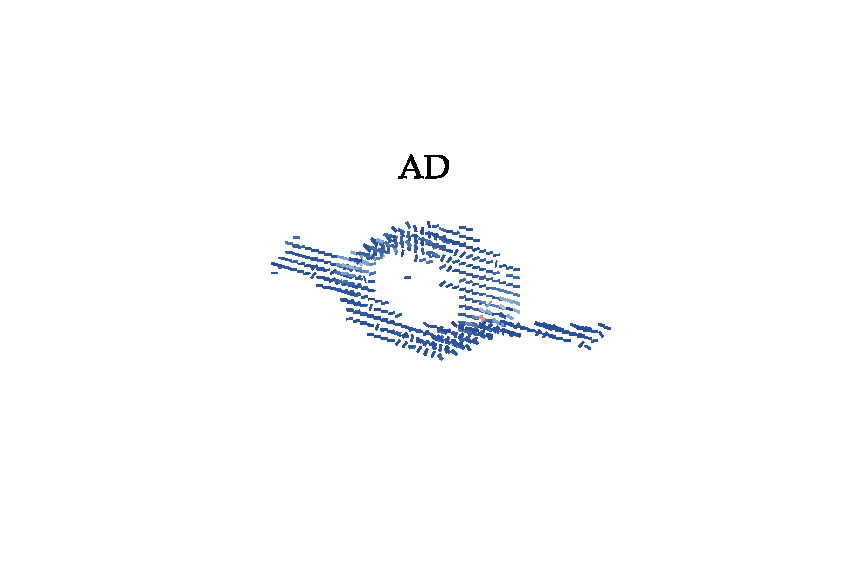
\includegraphics[trim={3.5cm 3.5cm 3.5cm 3.5cm},clip, width=10cm]{./svg-inkscape/ck_indAD_svg-tex.pdf} \\ \medskip % Picture

            \mySubtitle \\ \medskip % Thesis subtitle
            %\myDegree \\
            %\myDepartment \\
            %\myFaculty \\
            %\myUni \\ \bigskip

            \myTime\ -- \myVersion % Time and version

            \vfill

        \end{center}
    \end{addmargin}

\end{titlepage} % Main title page

% Back of the title page

\thispagestyle{empty}

\hfill

\vfill

\noindent\myName: \textit{\myTitle,} \mySubtitle, %\myDegree, 
\textcopyright\ \myTime

% You may wish to do something with the back of the title page, such as including your supervisors, location or time frame of the work. Below is an example of doing so although you may want to tweak it to your liking.

\bigskip

\noindent\spacedlowsmallcaps{Supervisors}: \\
\myProf \\
\myOtherProf \\ 
%\mySupervisor

%\medskip \\

%\noindent\spacedlowsmallcaps{Location}: \\
%\myLocation

%\medskip \\

%\noindent\spacedlowsmallcaps{Time Frame}: \\
%\myTime
 % Back of the title page

\cleardoublepage% Dedication

\thispagestyle{empty}
\refstepcounter{dummy}

\pdfbookmark[1]{Dedication}{Dedication} % Bookmark name visible in a PDF viewer

\vspace*{3cm}

\begin{center}
\emph{Ohana} means family. \\
Family means nobody gets left behind, or forgotten. \\ \medskip
--- Lilo \& Stitch    
\end{center}

\medskip

\begin{center}
Dedicated to the loving memory of Rudolf Miede. \\ \smallskip
1939\,--\,2005
\end{center}

% What is dedication? % Dedication page

%\cleardoublepage\include{FrontBackMatter/Foreword} % Uncomment and create a Foreword.tex to include a foreword

\cleardoublepage% Abstract

%\renewcommand{\abstractname}{Abstract} % Uncomment to change the name of the abstract

\pdfbookmark[1]{Abstract}{Abstract} % Bookmark name visible in a PDF viewer

\begingroup
\let\clearpage\relax
\let\cleardoublepage\relax
\let\cleardoublepage\relax

\chapter*{Abstract}
Short summary of the contents\dots a great guide by 
Kent Beck how to write good abstracts can be found here:  
\begin{center}
\url{https://plg.uwaterloo.ca/~migod/research/beckOOPSLA.html}
\end{center}

\endgroup			

\vfill % Abstract page

\cleardoublepage% Publications - a page listing research articles written using content in the thesis

\pdfbookmark[1]{Publications}{Publications} % Bookmark name visible in a PDF viewer

\chapter*{Publications} % Publications page text

Some ideas and figures have appeared previously in the following publications:\\

\noindent Put your publications from the thesis here. The packages \texttt{multibib} or \texttt{bibtopic} etc. can be used to handle multiple different bibliographies in your document.

%\begin{refsection}[ownpubs]
%    \small
%    \nocite{*} % is local to to the enclosing refsection
%    \printbibliography[heading=none]
%\end{refsection}

%\emph{Attention}: This requires a separate run of \texttt{bibtex} for your \texttt{refsection}, \eg, \texttt{ClassicThesis1-blx} for this file. You might also use \texttt{biber} as the backend for \texttt{biblatex}. See also \url{http://tex.stackexchange.com/questions/128196/problem-with-refsection}. % Publications from the thesis page

\cleardoublepage% Acknowledgements

\pdfbookmark[1]{Acknowledgements}{Acknowledgements} % Bookmark name visible in a PDF viewer

% \begin{flushright}{\slshape    
% We have seen that computer programming is an art, \\ 
% because it applies accumulated knowledge to the world, \\ 
% because it requires skill and ingenuity, and especially \\
% because it produces objects of beauty.} \\ \medskip
% --- \defcitealias{knuth:1974}{Donald E. Knuth}\citetalias{knuth:1974} \citep{knuth:1974}
% \end{flushright}

\bigskip

%----------------------------------------------------------------------------------------

\begingroup

\let\clearpage\relax
\let\cleardoublepage\relax
\let\cleardoublepage\relax

\chapter*{Acknowledgements}

% \noindent Put your acknowledgements here.\\
% 
% \noindent Many thanks to everybody who already sent me a postcard!\\
% 
% \noindent Regarding the typography and other help, many thanks go to Marco Kuhlmann, Philipp Lehman, Lothar Schlesier, Jim Young, Lorenzo Pantieri and Enrico Gregorio\footnote{Members of GuIT (Gruppo Italiano Utilizzatori di \TeX\ e \LaTeX )}, J\"org Sommer, Joachim K\"ostler, Daniel Gottschlag, Denis Aydin, Paride Legovini, Steffen Prochnow, Nicolas Repp, Hinrich Harms, Roland Winkler, and the whole \LaTeX-community for support, ideas and some great software.
% 
% \bigskip
% 
% \noindent\emph{Regarding \mLyX}: The \mLyX\ port was initially done by
% \emph{Nicholas Mariette} in March 2009 and continued by
% \emph{Ivo Pletikosi\'c} in 2011. Thank you very much for your work and the contributions to the original style.

\endgroup % Acknowledgements page

\pagestyle{scrheadings} % Show chapter titles as headings

\cleardoublepage% Table of Contents - List of Tables/Figures/Listings and Acronyms

\refstepcounter{dummy}

\pdfbookmark[1]{\contentsname}{tableofcontents} % Bookmark name visible in a PDF viewer

\setcounter{tocdepth}{2} % Depth of sections to include in the table of contents - currently up to subsections

\setcounter{secnumdepth}{3} % Depth of sections to number in the text itself - currently up to subsubsections

\manualmark
\markboth{\spacedlowsmallcaps{\contentsname}}{\spacedlowsmallcaps{\contentsname}}
\tableofcontents 
\automark[section]{chapter}
\renewcommand{\chaptermark}[1]{\markboth{\spacedlowsmallcaps{#1}}{\spacedlowsmallcaps{#1}}}
\renewcommand{\sectionmark}[1]{\markright{\thesection\enspace\spacedlowsmallcaps{#1}}}

\clearpage

\begingroup 
\let\clearpage\relax
\let\cleardoublepage\relax
\let\cleardoublepage\relax

%----------------------------------------------------------------------------------------
%	List of Figures
%----------------------------------------------------------------------------------------

\refstepcounter{dummy}
%\addcontentsline{toc}{chapter}{\listfigurename} % Uncomment if you would like the list of figures to appear in the table of contents
\pdfbookmark[1]{\listfigurename}{lof} % Bookmark name visible in a PDF viewer

\listoffigures

\vspace{8ex}
\newpage

%----------------------------------------------------------------------------------------
%	List of Tables
%----------------------------------------------------------------------------------------

\refstepcounter{dummy}
%\addcontentsline{toc}{chapter}{\listtablename} % Uncomment if you would like the list of tables to appear in the table of contents
\pdfbookmark[1]{\listtablename}{lot} % Bookmark name visible in a PDF viewer

\listoftables
        
\vspace{8ex}
\newpage
    
%----------------------------------------------------------------------------------------
%	List of Listings
%---------------------------------------------------------------------------------------- 

\refstepcounter{dummy}
%\addcontentsline{toc}{chapter}{\lstlistlistingname} % Uncomment if you would like the list of listings to appear in the table of contents
\pdfbookmark[1]{\lstlistlistingname}{lol} % Bookmark name visible in a PDF viewer

\lstlistoflistings 

\vspace{8ex}
\newpage
       
%----------------------------------------------------------------------------------------
%	Acronyms
%----------------------------------------------------------------------------------------

\refstepcounter{dummy}
%\addcontentsline{toc}{chapter}{Acronyms} % Uncomment if you would like the acronyms to appear in the table of contents
\pdfbookmark[1]{Acronyms}{acronyms} % Bookmark name visible in a PDF viewer

\markboth{\spacedlowsmallcaps{Acronyms}}{\spacedlowsmallcaps{Acronyms}}

\chapter*{Acronyms}

\begin{acronym}[UML]
\acro{DRY}{Don't Repeat Yourself}
\acro{API}{Application Programming Interface}
\acro{UML}{Unified Modeling Language}
\acro{FBP}{Filtered Back Projection}
\acro{CT}{Computed Tomography}
\acro{ML}{Maximum-Likelihood}
\acro{GD}{Gradient Descent}
\acro{CGD}{Conjugated Gradient Descent}
\acro{AD}{Automatic Differentiation}
\acro{SAXSTT}{Small Angle X-ray Scattering Tensor Tomography}
\acro{SH}{Spherical Harmonics}

\end{acronym}  
                   
\endgroup % Contents, list of figures/tables/listings and acronyms

\cleardoublepage

\pagenumbering{arabic} % Arabic page numbering for thesis content (1, 2, 3, etc)
%\setcounter{page}{90} % Uncomment to manually start the page counter at an arbitrary value (for example if you wish to count the pre-content pages in the page count)

\cleardoublepage % Avoids problems with pdfbookmark

%----------------------------------------------------------------------------------------
%	THESIS CONTENT - CHAPTERS
%----------------------------------------------------------------------------------------

%\ctparttext{You can put some informational part preamble text here. Illo principalmente su nos. Non message \emph{occidental} angloromanic da. Debitas effortio simplificate sia se, auxiliar summarios da que, se avantiate publicationes via. Pan in terra summarios, capital interlingua se que. Al via multo esser specimen, campo responder que da. Le usate medical addresses pro, europa origine sanctificate nos se.} % Text on the Part 1 page describing  the content in Part 1

%\ctparttext{\chapter{Introduction}

Machine learning has grown to be a powerful tool in many disciplines within physics. This includes computed tomography...}
%\ctparttext{Machine learning has grown to be a powerful tool in many disciplines within physics. This includes computed tomography...} Not include

\part{Introduction} %\part{Some Kind of Manual} % First part of the thesis

\chapter{Introduction}

Machine learning has grown to be a powerful tool in many disciplines within physics. This includes computed tomography... % Chapter 1

\cleardoublepage % Empty page before the start of the next part

%------------------------------------------------

\ctparttext{You can put some informational part preamble text here. Illo principalmente su nos. Non message \emph{occidental} angloromanic da. Debitas effortio simplificate sia se, auxiliar summarios da que, se avantiate publicationes via. Pan in terra summarios, capital interlingua se que. Al via multo esser specimen, campo responder que da. Le usate medical addresses pro, europa origine sanctificate nos se.} % Text on the Part 2 page describing the content in Part 2

\part{Review of The Literature}%\part{The Showcase} % Second part of the thesis

%
\chapter{Computed Tomography}

%RSD: Should do more precise calculations?
\section{X-rays}
X-rays are electromagnetic waves with energy in the orders of $keV$. From Planck's Equation \eqref{eq:Plancks_eq}, this corresponds to nanometer wavelengths. The equation relates energy of a photon $E$ to the frequency $\nu$ or wavelength $\lambda$ of the corresponding electromagnetic wave, as

\begin{equation}\label{eq:Plancks_eq}
    E = 2\pi \hbar \nu, \newline
    
    \nu = \frac{c}{\lambda},
\end{equation}
\noindent
with $c \sim 2.99776 \times 10^8 m/s$ being the speed of light \cite{blokhin1961physics}. The other constant is the reduced Planck's constant $\hbar \sim 1.0543 \times 10^{-34} Js$. 

Excitation, acceleration, and deceleration are the three most commonly utilised processes for producing X-rays. The first method is commonly referred to as "Characteristic X-ray radiation", which occurs when a highly energetic electron collides into a target atom. The accelerated electron transfers enough energy to eject an inner-shell electron from the atom. An outer electron may therefore occupy a lower-energy state. Due to conservation of energy, this process causes emission of a photon, as illustrated in Equation \eqref{eq:Char_radiation}. As the atomic energy levels are discrete, this process is characterised by a spectrum of discrete X-ray emission lines.
%\cite{Stark, G.. "X-ray." Encyclopedia Britannica, January 30, 2020. https://www.britannica.com/science/X-ray.}.  

\begin{equation}\label{eq:Char_radiation}
    E_{\mathrm{photon}} = - \Delta E = - (E_f - E_i)
\end{equation}

In addition to excitation, scattering events occur when electrons pass through an anode material. These events accelerate the electrons in a new direction, and X-rays known as $"Bremsstrahluhng"$ are emitted. % Include Intensity relation of Bremsstrahlung?

%Improve, Figure or equations
The synchrotron is the last common form of X-ray production, and is also based upon the principle of $"Bremsstrahluhng"$. Generally, charged particles are accelerated to very high energies, and magnets maintain their circular path. As moving objects in a circular path experience a centrifugal acceleration perpendicular to its directions, $"Bremsstrahluhng"$ X-rays are emitted. 
%\cite{Britannica, T. Editors of Encyclopaedia. "synchrotron." Encyclopedia Britannica, February 7, 2018. https://www.britannica.com/technology/synchrotron.}

\section{Beer-Lambert's Law}
The intensity of X-rays attenuates upon interacting with matter. This is due to photoelectric absorption, elastic Rayleigh scattering, and inelastic Compton scattering. The attenuation coefficient $\mu$ describes this attenuation in an inhomogeneous sample as
% Include formulas for scattering processes?

\begin{equation}
    I(s) = I(0) \exp(- \int_{0}^{s} \mu(\nu) d\nu),
\end{equation}
\noindent
where $s$ is the distance from the initial intensity to the end of the sample, effectively the thickness of the sample, and $I(0)$ is the initial intensity. Here, the spectral dependence, $\mu(E,\nu)$ is often neglected as it is unknown \cite{buzug2009computed}. A simple manipulation of the expression gives the projection line integral

\begin{equation}\label{eq:projection}
    p(s) = -\ln(\frac{I(s)}{I(0)} ) = \int_{0}^{s} \mu(\nu) d\nu.
\end{equation}

\section{Radon Transform}
The projection line integral in Equation \eqref{eq:projection} may be viewed as a Radon transform of an object function $f(x,y)$ for a single orientation $\theta$ \cite{zeng2010medical}. Confidence in this statement may be achieved by comparing Equation \eqref{eq:projection} with a single-angle Radon transform \eqref{eq:Radon_transform}

\begin{equation}\label{eq:Radon_transform}
    p_{\theta}(r) = \int_{-\infty}^{\infty} f(r,\nu) d\nu.
\end{equation}

%\section{Detectors}??? Cannot be relevant

\section{Fourier Slice Theorem}
%\section{Projections}
The key in computed tomography is to determine the spatial dependence of the attenuation coefficient. By sampling many projections, meaning line integrals from different orientations and crossections, data necessary to reconstruct a three-dimensional image is collected. For a given crossection of the object $f(x,y)$, the detected intensity is plotted as a function of projection number and pixel number in what is called a sinogram. By utilising this sinogram and the Fourier slice theorem, the object $f(x,y)$ may be determined by other means than computing the full inverse Radon transform.

%\section{Fourier Slice Theorem}

The Fourier slice theorem states that the full 2D Fourier transform $F(\omega_x, \omega_y)$ of an object $f(x,y)$ can be constructed from a series of 1D Fourier transforms $P(\omega)$ of projections $p(s)$ with different orientations \cite{zeng2010medical}. 
%  that the 1D Fourier transform $P(\omega)$ of the projection $p(s)$ of the object $f(x,y)$ is equal to a slice through the origin of the 2D Fourier transform $F(\omega_x, \omega_y)$ \cite{}. 


% ILLUSTRATE with a Figure
%See and reconstruct Figure 5.13 in buzug2009computed possibly... or the one in zeng2010medical


\section{Filtered Back Projection}
In short, the filtered back projection (FBP) algorithm reconstructs the object by forward and inverse Fourier transforms. Firstly, the sinogram of projections is mapped to frequency space in polar coordinates by subsequent 1D Fourier transforms, as shown in Equation \eqref{eq:FBP_1}:

\begin{equation}\label{eq:FBP_1}
    P(\theta, \omega) = \int_{-\infty}^{\infty} p(\theta,r)e^{-2\pi i\omega r} dr.
\end{equation}

With this the 2D Fourier transform $F(u,v)$ of the object $f(x,y)$ is found. The final step is an inverse 2D Fourier transform with a $ramp$-filter of $|\omega|$ to account for the radial distribution of points in polar coordinates. This filter is also the Jacobian of the area integration element in the polar Fourier space. Consequently, the object function can be expressed as

\begin{equation}
    f(x,y) = \int_{0}^{\pi} \int_{-\infty}^{\infty} \left|\omega\right| P(\theta,\omega)e^{-2\pi i\omega (x\cos\theta - y\sin\theta)} d\omega d\theta.
\end{equation}

%RSD: Read through a couple of times. 







%\include{2.Teil Theory/02TheorySAXSTT} 
%\include{2.Teil Theory/03MachineLearning} 
%\include{2.Teil Theory/04GradientDescent}
%\include{2.Teil Theory/05TheoryAutodiff}
% This is many chapters. Instead, one chapter on the image technique and one on the optimalisation?

\chapter{Computed Tomography}

%RSD: Should do more precise calculations?
\section{X-rays}
X-rays are electromagnetic waves with energy in the orders of $keV$. From Planck's Equation \eqref{eq:Plancks_eq}, this corresponds to nanometer wavelengths. The equation relates energy of a photon $E$ to the frequency $\nu$ or wavelength $\lambda$ of the corresponding electromagnetic wave, as

\begin{equation}\label{eq:Plancks_eq}
    E = 2\pi \hbar \nu, \newline
    
    \nu = \frac{c}{\lambda},
\end{equation}
\noindent
with $c \sim 2.99776 \times 10^8 m/s$ being the speed of light \cite{blokhin1961physics}. The other constant is the reduced Planck's constant $\hbar \sim 1.0543 \times 10^{-34} Js$. 

Excitation, acceleration, and deceleration are the three most commonly utilised processes for producing X-rays. The first method is commonly referred to as "Characteristic X-ray radiation", which occurs when a highly energetic electron collides into a target atom. The accelerated electron transfers enough energy to eject an inner-shell electron from the atom. An outer electron may therefore occupy a lower-energy state. Due to conservation of energy, this process causes emission of a photon, as illustrated in Equation \eqref{eq:Char_radiation}. As the atomic energy levels are discrete, this process is characterised by a spectrum of discrete X-ray emission lines.
%\cite{Stark, G.. "X-ray." Encyclopedia Britannica, January 30, 2020. https://www.britannica.com/science/X-ray.}.  

\begin{equation}\label{eq:Char_radiation}
    E_{\mathrm{photon}} = - \Delta E = - (E_f - E_i)
\end{equation}

In addition to excitation, scattering events occur when electrons pass through an anode material. These events accelerate the electrons in a new direction, and X-rays known as $"Bremsstrahluhng"$ are emitted. % Include Intensity relation of Bremsstrahlung?

%Improve, Figure or equations
The synchrotron is the last common form of X-ray production, and is also based upon the principle of $"Bremsstrahluhng"$. Generally, charged particles are accelerated to very high energies, and magnets maintain their circular path. As moving objects in a circular path experience a centrifugal acceleration perpendicular to its directions, $"Bremsstrahluhng"$ X-rays are emitted. 
%\cite{Britannica, T. Editors of Encyclopaedia. "synchrotron." Encyclopedia Britannica, February 7, 2018. https://www.britannica.com/technology/synchrotron.}

\section{Beer-Lambert's Law}
The intensity of X-rays attenuates upon interacting with matter. This is due to photoelectric absorption, elastic Rayleigh scattering, and inelastic Compton scattering. The attenuation coefficient $\mu$ describes this attenuation in an inhomogeneous sample as
% Include formulas for scattering processes?

\begin{equation}
    I(s) = I(0) \exp(- \int_{0}^{s} \mu(\nu) d\nu),
\end{equation}
\noindent
where $s$ is the distance from the initial intensity to the end of the sample, effectively the thickness of the sample, and $I(0)$ is the initial intensity. Here, the spectral dependence, $\mu(E,\nu)$ is often neglected as it is unknown \cite{buzug2009computed}. A simple manipulation of the expression gives the projection line integral

\begin{equation}\label{eq:projection}
    p(s) = -\ln(\frac{I(s)}{I(0)} ) = \int_{0}^{s} \mu(\nu) d\nu.
\end{equation}

\section{Radon Transform}
The projection line integral in Equation \eqref{eq:projection} may be viewed as a Radon transform of an object function $f(x,y)$ for a single orientation $\theta$ \cite{zeng2010medical}. Confidence in this statement may be achieved by comparing Equation \eqref{eq:projection} with a single-angle Radon transform \eqref{eq:Radon_transform}

\begin{equation}\label{eq:Radon_transform}
    p_{\theta}(r) = \int_{-\infty}^{\infty} f(r,\nu) d\nu.
\end{equation}

%\section{Detectors}??? Cannot be relevant

\section{Fourier Slice Theorem}
%\section{Projections}
The key in computed tomography is to determine the spatial dependence of the attenuation coefficient. By sampling many projections, meaning line integrals from different orientations and crossections, data necessary to reconstruct a three-dimensional image is collected. For a given crossection of the object $f(x,y)$, the detected intensity is plotted as a function of projection number and pixel number in what is called a sinogram. By utilising this sinogram and the Fourier slice theorem, the object $f(x,y)$ may be determined by other means than computing the full inverse Radon transform.

%\section{Fourier Slice Theorem}

The Fourier slice theorem states that the full 2D Fourier transform $F(\omega_x, \omega_y)$ of an object $f(x,y)$ can be constructed from a series of 1D Fourier transforms $P(\omega)$ of projections $p(s)$ with different orientations \cite{zeng2010medical}. 
%  that the 1D Fourier transform $P(\omega)$ of the projection $p(s)$ of the object $f(x,y)$ is equal to a slice through the origin of the 2D Fourier transform $F(\omega_x, \omega_y)$ \cite{}. 


% ILLUSTRATE with a Figure
%See and reconstruct Figure 5.13 in buzug2009computed possibly... or the one in zeng2010medical


\section{Filtered Back Projection}
In short, the filtered back projection (FBP) algorithm reconstructs the object by forward and inverse Fourier transforms. Firstly, the sinogram of projections is mapped to frequency space in polar coordinates by subsequent 1D Fourier transforms, as shown in Equation \eqref{eq:FBP_1}:

\begin{equation}\label{eq:FBP_1}
    P(\theta, \omega) = \int_{-\infty}^{\infty} p(\theta,r)e^{-2\pi i\omega r} dr.
\end{equation}

With this the 2D Fourier transform $F(u,v)$ of the object $f(x,y)$ is found. The final step is an inverse 2D Fourier transform with a $ramp$-filter of $|\omega|$ to account for the radial distribution of points in polar coordinates. This filter is also the Jacobian of the area integration element in the polar Fourier space. Consequently, the object function can be expressed as

\begin{equation}
    f(x,y) = \int_{0}^{\pi} \int_{-\infty}^{\infty} \left|\omega\right| P(\theta,\omega)e^{-2\pi i\omega (x\cos\theta - y\sin\theta)} d\omega d\theta.
\end{equation}

%RSD: Read through a couple of times. 







\chapter{Machine Learning Optimisation}

\section{Maximum Likelihood Estimation}

The maximum likelihood estimator is defined to be the set of parameters $\bm{\theta}_{ML}$ that maximise the probability $P(\bm{y}\left | \right \bm{x}; \bm{\theta})$. In other words, it chooses the parameters that produce the most probable estimation $\bm{\hat{y}}$ of the true output $\bm{y}$ given the input $\bm{x}$. Equation \eqref{eq:Max_likelihood} defines this mathematically \cite{Goodfellow-et-al-2016}.

\begin{equation}\label{eq:Max_likelihood}
     \bm{\theta}_{ML} = \argmax_{\bm{\theta}} P(\bm{y}\left | \right \bm{x}; \bm{\theta})
\end{equation}

ML estimation is an example of supervised learning, because the true output, the targets are known. In supervised learning, the estimation is evaluated by computing the error relative to the true output. The expression for the total error of the model is called the cost function $J(\bm{\theta})$, which is a sum of loss functions $\mathcal{L}(\bm{y},\bm{\hat{y}} )$ representing the error of a single data point. 

\section{Gradient Descent}

Gradient descent is an optimisation algorithm that updates the model's parameters based on the gradient of the cost function and the step size $\alpha$, as shown in Equation \eqref{eq:GD} \cite{ruder2016overview}.

\begin{equation}\label{eq:GD}
    \bm{\theta} = \bm{\theta} - \alpha \bm{\nabla_{\theta}} J(\bm{\theta})
\end{equation}

The idea of this algorithm is that by following the gradient of the cost function, it is possible to find the global, or at least a sufficiently good local, minima in parameter space. In this way, the estimation will converge and minimise the error. Gradient descent in parameter space is visualised in Figure \ref{fig:GD_surface} 
% Matplotlib surface plot with path. + Make gif. 

\begin{figure}
    \centering
    \includegraphics{}
    \caption{A surface plot of the space of error for a model. The trajectory shows the path of parameter optimisation based on gradient descent}
    \label{fig:GD_surface}
\end{figure}

\section{Conjugate Gradient Descent}

%There are several optimisation algorithms that are based on GD, for instance stochastic gradient descent (SGD) and conjugate gradient descent (CGD). The latter is shortly summarised composed of determination of steepest descent, a line search to find an appropiate step size $\alpha$, and the completion of a step. 

The basic gradient descent algorithm is prone to require many iterations before converging. When solving computationally expensive optimisation tasks using gradient descent, one should therefore consider to use a variant such as Conjugate Gradient Descent (CGD). This method serves as a compromise between basic first order gradient descent, which is also referred to as "steepest descent", and Newton's second order method. The latter uses the Hessian to converge in a small number of highly expensive iterations.

%Consider illustrating the Hessian and/or the Jacobian

% Some equations regarding CGD... Do not now it that well.


\section{Automatic Differentiation}


\chapter{Scattering of X-rays}

\section{Coherent X-ray Beam}

\section{X-ray Diffraction / Fraunhofer Diffraction} %Which to describe?

\section{Reciprocal Space Related to Electron Density}

\chapter{Small Angle X-ray Scattering Tensor Tomography}

\section{Experimental Setup}

\section{Modelling of Anisotropic Scattering}

\section{Optimisation Algorithm}


\cleardoublepage % Empty page before the start of the next part


\part{Methods}
\chapter{Data Sets} % or Original set up and include 

\section{Carbon Knot from Synchrotron Measurement}

%\section{Reconstruction Algorithm} %RSD: Ish

%\section{Spherical Harmonics Reconstruction Parameters}

%\section{Alternative Reconstruction Parameters}

% Include the parts about the reconstruction here or 



\chapter{Implementation}

%\section{Description of SASTT Package from Paul Scherrer Institut} ?
\section{Proof of Concept Automatic Differentiation}

\section{Optimisation Using Symbolic Gradients}

\section{Automatic Differentiation in MATLAB}%?

\section{Automatic Differentiation Using Pytorch}%?



\chapter{Calculations}

\section{Gradients of Alternative Functional} %Functional is function of functions

\section{Reconstruction of Known Model Using Automatic Differentiation SAXSTT}

\section{Comparison of Automatic and Symbolic Differentiation for SAXSTT Applied to Known Model}

% All included in results should be mentioned here, But may be located in separate chapters in results?

\cleardoublepage



\part{Results}
\chapter{Disproval of Derived Symbolic Gradients}
\chapter{Performed Reconstructions }
\chapter{Computation Performance}

\cleardoublepage


\part{Discussion}

\chapter{Validation of SAXSTT Algorithms}
\chapter{Comparison of Symbolic and Automatic Gradients}
\chapter{Improvements of Computational Performance}

\cleardoublepage

%----------------------------------------------------------------------------------------
%	THESIS CONTENT - APPENDICES
%----------------------------------------------------------------------------------------

\appendix

\part{Appendix} % New part of the thesis for the appendix

% Appendix A

\chapter{Appendix Test}

%----------------------------------------------------------------------------------------

\lipsum[13-14]

%----------------------------------------------------------------------------------------

\section{Appendix Section Test}
\lipsum[15]

\graffito{More dummy text}
\lipsum[16]

%----------------------------------------------------------------------------------------

\section{Another Appendix Section Test}
\lipsum[17]

\begin{table}
\myfloatalign
\begin{tabularx}{\textwidth}{Xll} \toprule
\tableheadline{labitur bonorum pri no} & \tableheadline{que vista}
& \tableheadline{human} \\ \midrule
fastidii ea ius & germano &  demonstratea \\
suscipit instructior & titulo & personas \\
\midrule
quaestio philosophia & facto & demonstrated \\
\bottomrule
\end{tabularx}
\caption[Autem usu id]{Autem usu id.}
\label{tab:moreexample}
\end{table}

\lipsum[18]

There is also a useless Pascal listing below: \autoref{lst:useless}.

\begin{lstlisting}[float=b,language=Pascal,frame=tb,caption={A floating example (\texttt{listings} manual)},label=lst:useless]
for i:=maxint downto 0 do
begin
{ do nothing }
end;
\end{lstlisting} % Appendix A
%% Appendix X

\chapter{Appendix Title}

%----------------------------------------------------------------------------------------

% Content begins here % Appendix B - empty template

%----------------------------------------------------------------------------------------
%	POST-CONTENT THESIS PAGES
%----------------------------------------------------------------------------------------

\cleardoublepage% Bibliography

\label{app:bibliography} % Reference the bibliography elsewhere with \autoref{app:bibliography}

\manualmark % Work-around to have small caps also here in the headline
\markboth{\spacedlowsmallcaps{\bibname}}{\spacedlowsmallcaps{\bibname}} % Work-around to have small caps also
%\phantomsection
\refstepcounter{dummy}

\addtocontents{toc}{\protect\vspace{\beforebibskip}} % Place the bibliography slightly below the rest of the document content in the table of contents
\addcontentsline{toc}{chapter}{\tocEntry{\bibname}}

\printbibliography % Bibliography

\cleardoublepage% Declaration

\refstepcounter{dummy}
\pdfbookmark[0]{Declaration}{declaration} % Bookmark name visible in a PDF viewer

\chapter*{Declaration} % Declaration section text

\thispagestyle{empty}

Put your declaration here.
\bigskip
 
\noindent\textit{\myLocation, \myTime}

\smallskip

\begin{flushright}
\begin{tabular}{m{5cm}}
\\ \hline
\centering\myName \\
\end{tabular}
\end{flushright}
 % Declaration

\cleardoublepage% Colophon (a brief description of publication or production notes relevant to the edition)

\pagestyle{empty}

\hfill

\vfill

\pdfbookmark[0]{Colophon}{colophon}

\section*{Colophon}

This document was typeset using the typographical look-and-feel \texttt{classicthesis} developed by Andr\'e Miede. The style was inspired by Robert Bringhurst's seminal book on typography ``\emph{The Elements of Typographic Style}''.

\bigskip

\noindent\finalVersionString % Colophon

%----------------------------------------------------------------------------------------

\end{document}
